\documentclass[a4paper]{beamer}
\usepackage{tikz}
\usetheme{Berlin}
\title{Introduction to the \texttt{nom} crate}
\subtitle{Rust Berlin Online Meetup}
\date{8.11.2022}
\author{Jörn Bethune}

\begin{document}

\begin{frame}
\maketitle
\end{frame}

\section{Trees}

\begin{frame}\frametitle{Short interlude about Trees in Computing}

\begin{columns}

\begin{column}{.5\textwidth}
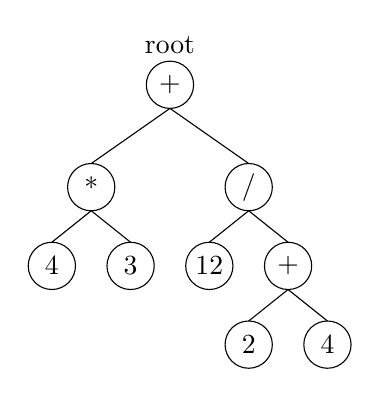
\begin{tikzpicture}
\draw (7,0) circle (3mm);
\draw (7,0.5) node{root};
\draw (7,0) node{+};
\draw (7,-0.3) -- (6,-1);
\draw (7,-0.3) -- (8,-1);

\draw (6,-1.3) circle (3mm);
\draw (6,-1.3) node{*};

\draw (8,-1.3) circle (3mm);
\draw (8,-1.3) node{/};

\draw (6,-1.6) -- (5.5,-2);
\draw (6,-1.6) -- (6.5,-2);

\draw (8,-1.6) -- (7.5,-2);
\draw (8,-1.6) -- (8.5,-2);

\draw (5.5, -2.3) circle (3mm);
\draw (5.5, -2.3) node{4};

\draw (6.5, -2.3) circle (3mm);
\draw (6.5, -2.3) node{3};

\draw (7.5, -2.3) circle (3mm);
\draw (7.5, -2.3) node{12};

\draw (8.5, -2.3) circle (3mm);
\draw (8.5, -2.3) node{+};

\draw (8.5, -2.6) -- (8,-3);
\draw (8.5, -2.6) -- (9,-3);

\draw (8, -3.3) circle (3mm);
\draw (8, -3.3) node{2};

\draw (9, -3.3) circle (3mm);
\draw (9, -3.3) node{4};
\end{tikzpicture}
\end{column}

\begin{column}{.5\textwidth}
\begin{itemize}
 \item A lot of calculations can be represted as trees.
 \item Here we have a \emph{binary} tree representing the calculation $4 * 3 + 12 / (2 + 4)$
 \item Storing calculations (or, more general, operations) in a tree takes care of operator precedence (multiplication has a higher priority than addition).
\end{itemize}
\end{column}

\end{columns}
\end{frame}

\begin{frame}\frametitle{Building trees}
\begin{itemize}
 \item Many file formats are hierarchical in nature. For example: HTML (<html>, <head>, <body>, ...)
 \item But also most software code is organised in hierarchies: Modules, classes, functions \& methods, parameters, variables, operations
 \item Trees are a very fitting data structure to work with hierarchical data.
\end{itemize}
\end{frame}

\section{nom}
\subsection{what is it?}

\begin{frame}\frametitle{What problems does nom solve?}
\begin{columns}
\begin{column}{.3\textwidth}
\includegraphics[scale=0.5]{nom.png}
\end{column}
\begin{column}{.7\textwidth}
\begin{itemize}
\item Nom is a parser combinator: You can combine several sub-parsers into larger ones
\item Reading data in different formats can be tricky when the structure is complex
\item Nom looks at data by trying different parsers until one matches
\item And when data is successfully parsed, you typically want to convert it into your own Rust type
%\item Rust is kind of like the deserialization part of Serde, but the file format is not predefined
\end{itemize}
\end{column}
\end{columns}

\end{frame}

\subsection{how to use it?}

\begin{frame}[fragile]\frametitle{Trying to eat the input}
\begin{semiverbatim}
type Err = nom::error::Error<&'static str>;
use nom::branch::alt;
use nom::character::complete::char;\uncover<2->{
let mut operator_parser = alt((
    char::<&str, Err>('+'),
    char('-'),
    char('*'), // each of these returns a Rust char
    char('/'),
));}\uncover<4->{
if let Ok((tail, op_char)) = }\uncover<3->{operator_parser("* 42 bla")}\uncover<4->{ \{
    assert_eq!(op_char, '*');
    assert_eq!(tail, " 42 bla");
\}}
\end{semiverbatim}
\end{frame}

\begin{frame}[fragile]\frametitle{IResult}
\begin{semiverbatim}
use nom::\{Needed, error::Error\};

type IResult<I, O, E = Error<I>> = Result<(I, O), Err<E>>;

enum Err<E> \{
  Incomplete(Needed),
  Error(E),
  Failure(E),
\}
\end{semiverbatim}

Nom uses generic data types to offer its users high flexibility.
But that also means that types can get confusing.
\end{frame}

\begin{frame}[fragile]\frametitle{Typechecks still need to be satisfied!}
\begin{semiverbatim}
enum FlyingThing \{
    Bird,
    Plane,
    Superman,
\}
let parser = alt((
    bird_parser,
    plane_parser,
    superman_parser));

let (tail, flything) = map_res(parser,
                               |x| x.try_into())(input)?;
\end{semiverbatim}
\end{frame}

\end{document}
